\documentclass{article}

\usepackage[utf8]{inputenc}
\usepackage[T1]{fontenc}
\usepackage{lipsum}
\usepackage{graphicx}
\usepackage{amsmath}
\usepackage[margin=1in]{geometry}
\usepackage{titlesec}

\titleformat{\section}
{\LARGE\bfseries}{\thesection}{1em}{}

\titleformat{\subsection}
{\Large\bfseries}{\thesection}{1em}{}

\begin{document}

\pagestyle{empty}

\section*{Diagramma delle classi}
\large

\textbf{Detto anche diagramma di dominio}
\begin{center}
    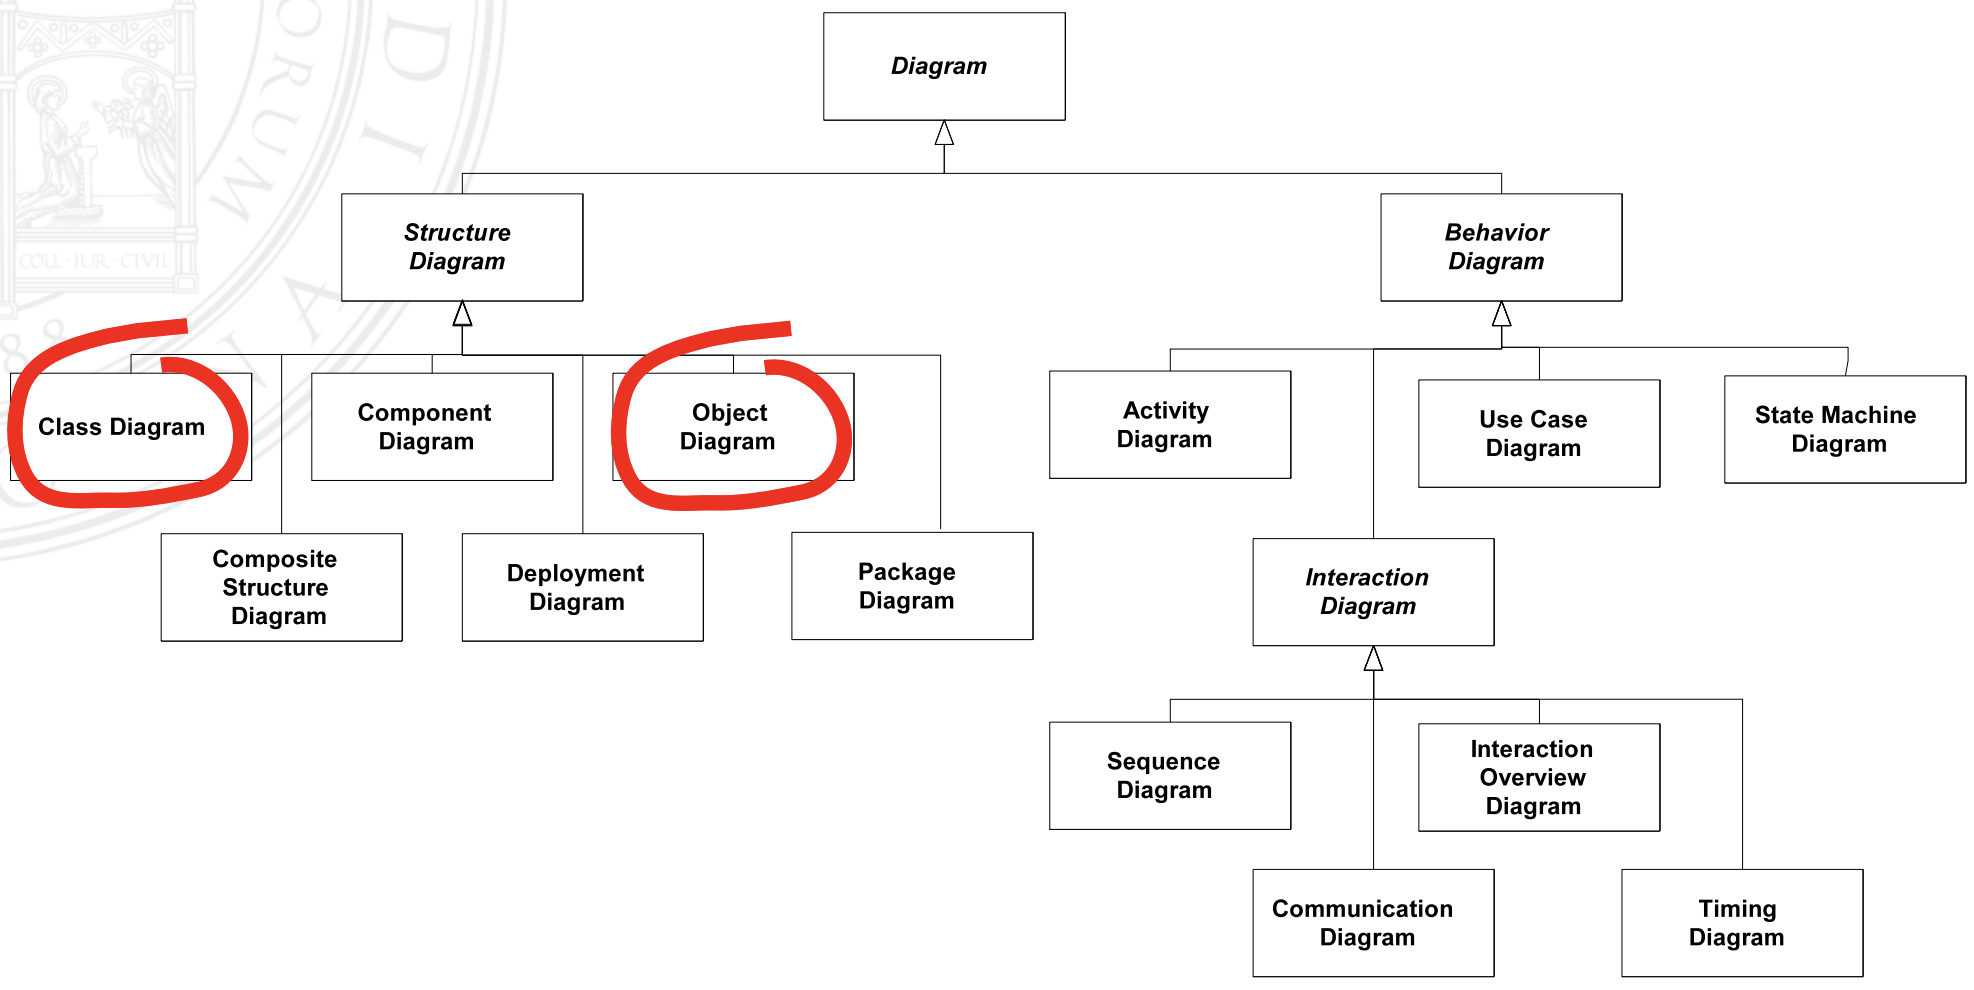
\includegraphics[width=1\textwidth]{foto 1.png}
\end{center}
\textit{Nota Bene}: si considera anche \textit{Object Diagram}, essendo molto simile al diagramma delle classi ma considerando le singole istanze. \vspace{14pt}\\
Una classe è un tipo che rappresenta oggetti che condividono caratteristiche comuni.
Viene raffigurata come un rettangolo dal contorno solido con il nome della classe al suo interno ed è potenzialmente divisa in compartimenti separati da linee orizzontali sotto il nome.
I compartimenti tipici sono il compartimento delle \textit{operazioni} e il compartimento degli \textit{attributi}.
Alcuni esempi di rappresentazione grafica di una classe, con diversi livelli di complessità:
\begin{center}
    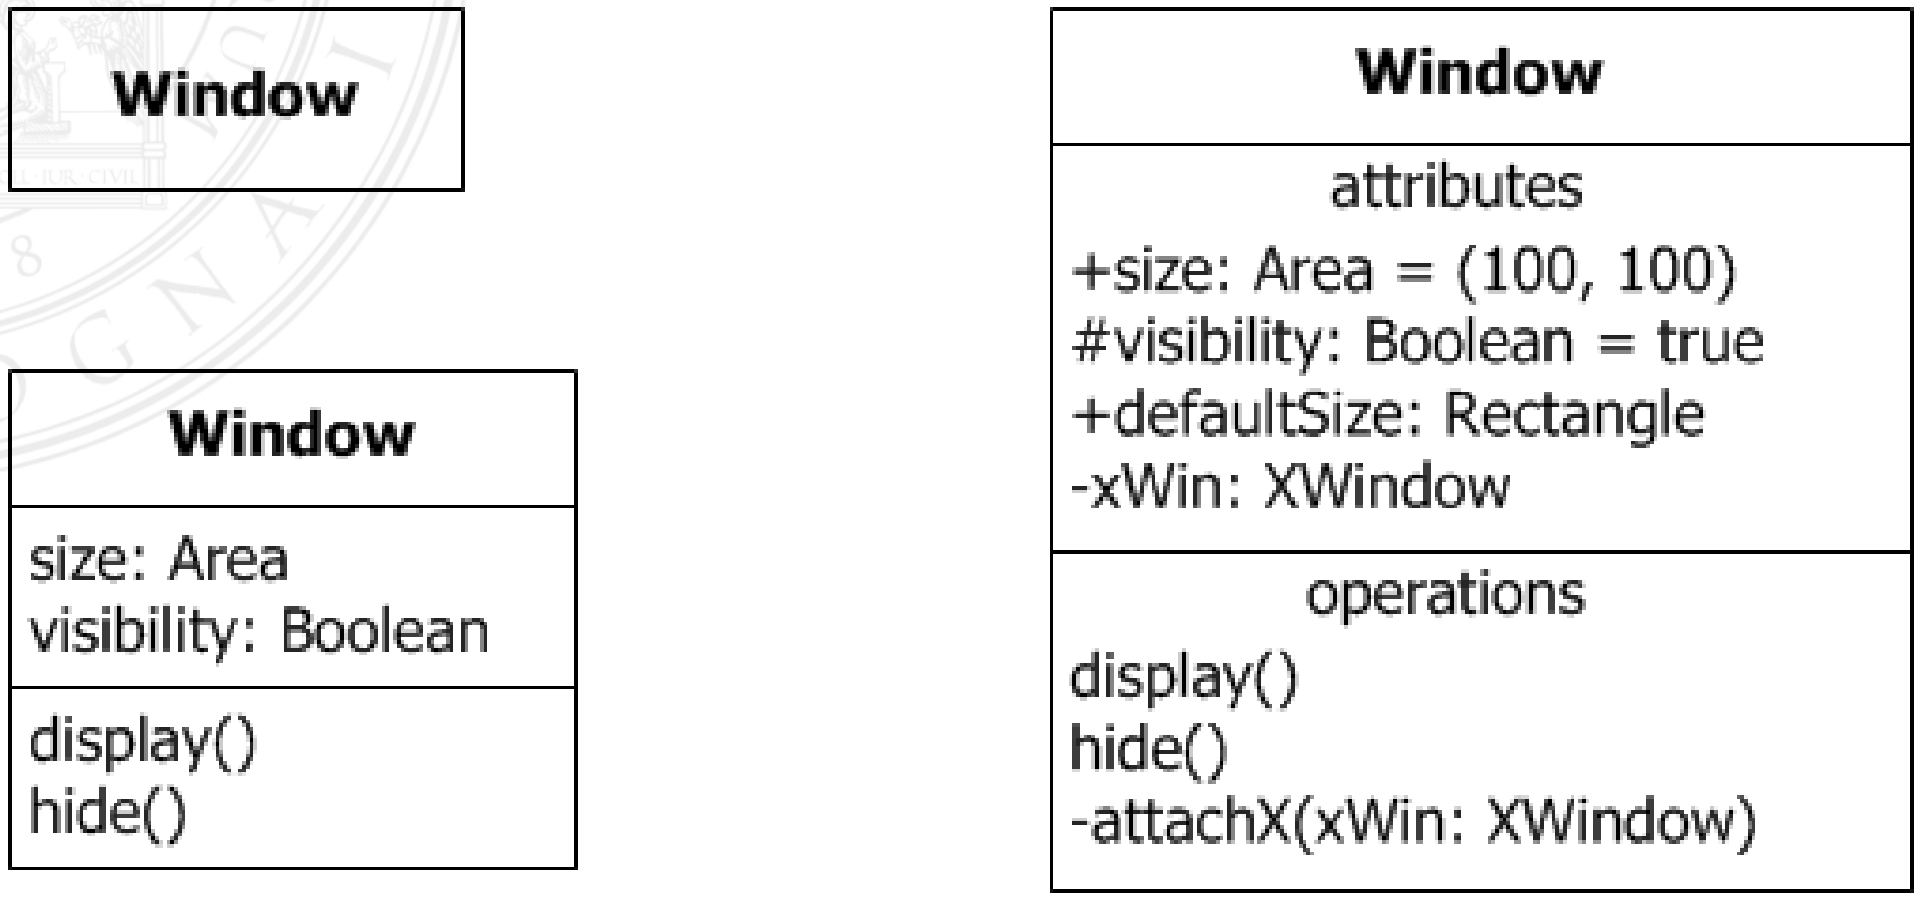
\includegraphics[width=0.7\textwidth]{foto 2.png}
\end{center}

\subsection*{Proprietà e operazioni}
\large

Le \textbf{proprietà} sono caratteristiche strutturali di una classe. Una sintassi semplificata può essere:
\begin{center}
    \textbf{[+,-,\#,\texttildelow][/]<name>[:<type>][<mult>]}
\end{center}
Le \textbf{operazioni} sono caratteristiche comportamentali di una classe. Una sintassi semplificata può essere:
\begin{center}
    \textbf{[+,-,\#,\texttildelow]<name>[<params>][:<type>]}
\end{center}
In entrambi i casi, il nome è \textbf{obbligatorio}, mentre i valori inclusi in \textbf{[]} sono \textbf{opzionali}.

\subsection*{Visibilità}
\large
\begin{enumerate}
    \renewcommand{\labelenumi}{-}
    \item \textbf{+}: \textit{public}, visibile a tutti
    \item \textbf{-}: \textit{private}, visibile soltanto nel suo ambiente
    \item \textbf{\#}: \textit{protected}, visibile agli elementi che possiedono una relazione di generalizzazione
    \item \textbf{\texttildelow}: \textit{package}, visible a tutti gli elementi nel package
\end{enumerate}

\subsection*{Moltiplicità}
\large
\begin{center}
    \textbf{<multiplicity-range> ::= [<lower>...] <upper>}
\end{center}
In questo caso, in presenza di \textbf{*}, si considera un limite superiore infinito. Vengono spesso utilizzate per indicare la moltiplicità i seguenti valori:
\begin{enumerate}
    \renewcommand{\labelenumi}{-}
    \item \textbf{1}: esattamente 1
    \item \textbf{0...1}: potrebbe non essere presente, o essere presente una sola volta
    \item \textbf{1...*}: potrebbe esserne presente uno solo, o non si sa di preciso la quantità
    \item \textbf{*}: non si sa di preciso la quantità
\end{enumerate}

\subsection*{Istanze}
\large

Le \textbf{istanze} (o \textbf{oggetti}) sono, insomma, delle istanze. Obbediscono alla \textbf{struttura della classe} della quale sono una istanza.
Gli oggetti di una classe devono avere un valore per ogni attributo che fa parte di quella classe, seguendo le caratteristiche dell'attributo, come il tipo e la moltiplicità. \\
La notazione grafica è simile a quella delle classi ma il nome compare sottolineato ed è una concatenazione del nome dell'istanza (se presente), due punti (':') e la classe della quale è una istanza. 
\begin{center}
    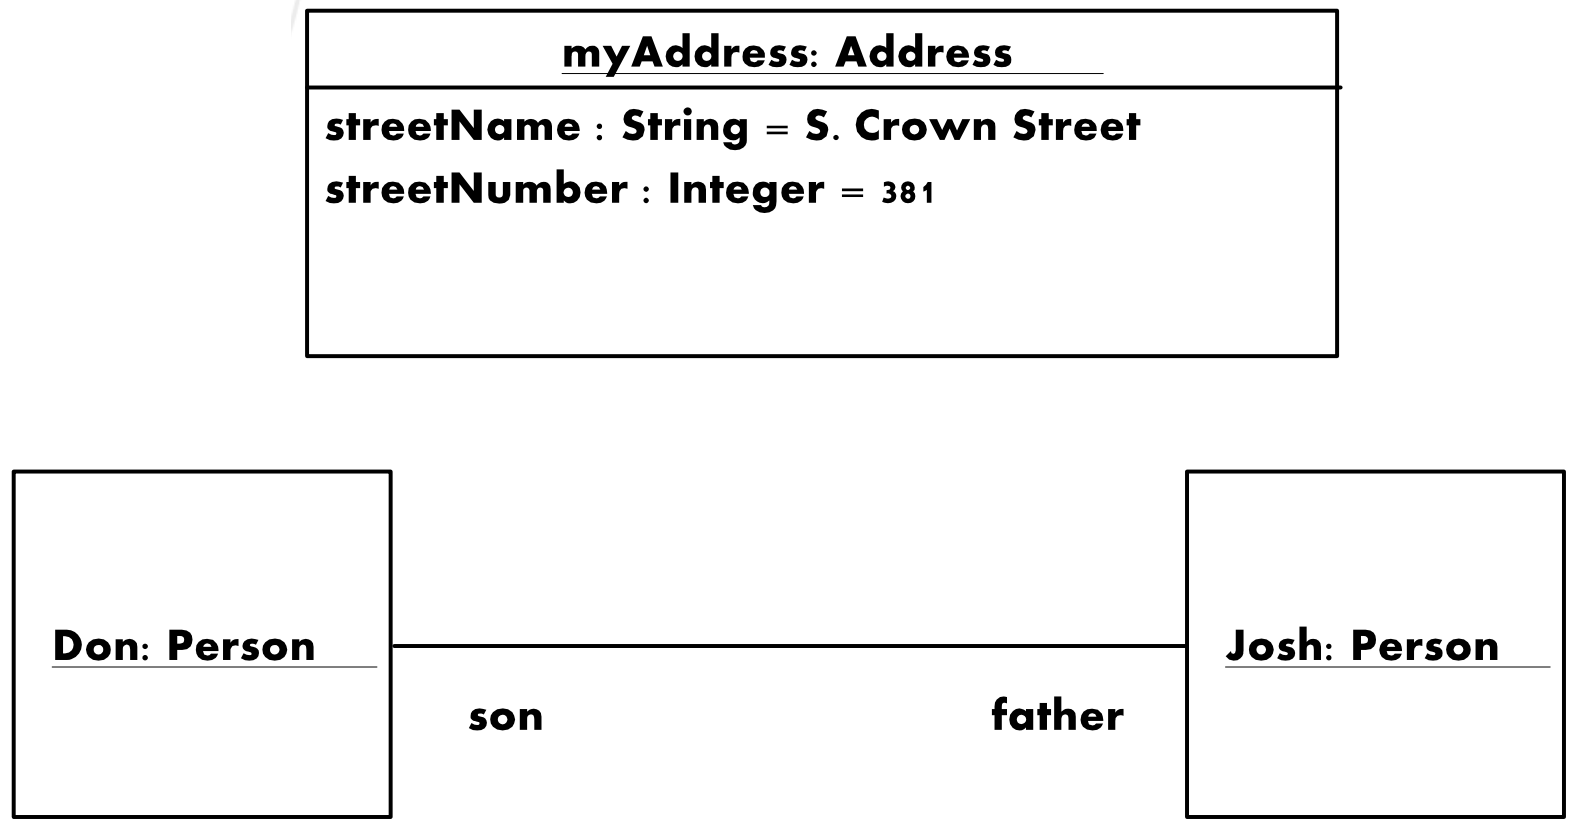
\includegraphics[width=0.6\textwidth]{foto 3.png}
\end{center}

\subsection*{Relazioni}
\large

Molte relazioni possono essere rappresentate in diagramma di classi:
\begin{enumerate}
    \renewcommand{\labelenumi}{-}
    \item \textbf{Generalizzazione}
    \item \textbf{Dipendenza}
    \item \textbf{Realizzazione}
    \item \textbf{Associazione}
    \item \textbf{Aggregazione}
    \item \textbf{Composizione}
\end{enumerate}

\subsection*{Generalizzazione/specializzazione}
\large

\textbf{Generalizzazione/specializzazione} sono concetti di base nel modello \textit{MOF} che assuomono un comportamento più dettagliato quando utilizzato tra classi. Ogni generalizzazione mette in relazione una specifica classe con una classe più generale con un meccanismo simile all'ereditarietà. Esiste una relazione "\textit{is-a}" tra i due elementi, corrispondente all'ereditarietà nei linguaggi di programmazione.
\begin{center}
    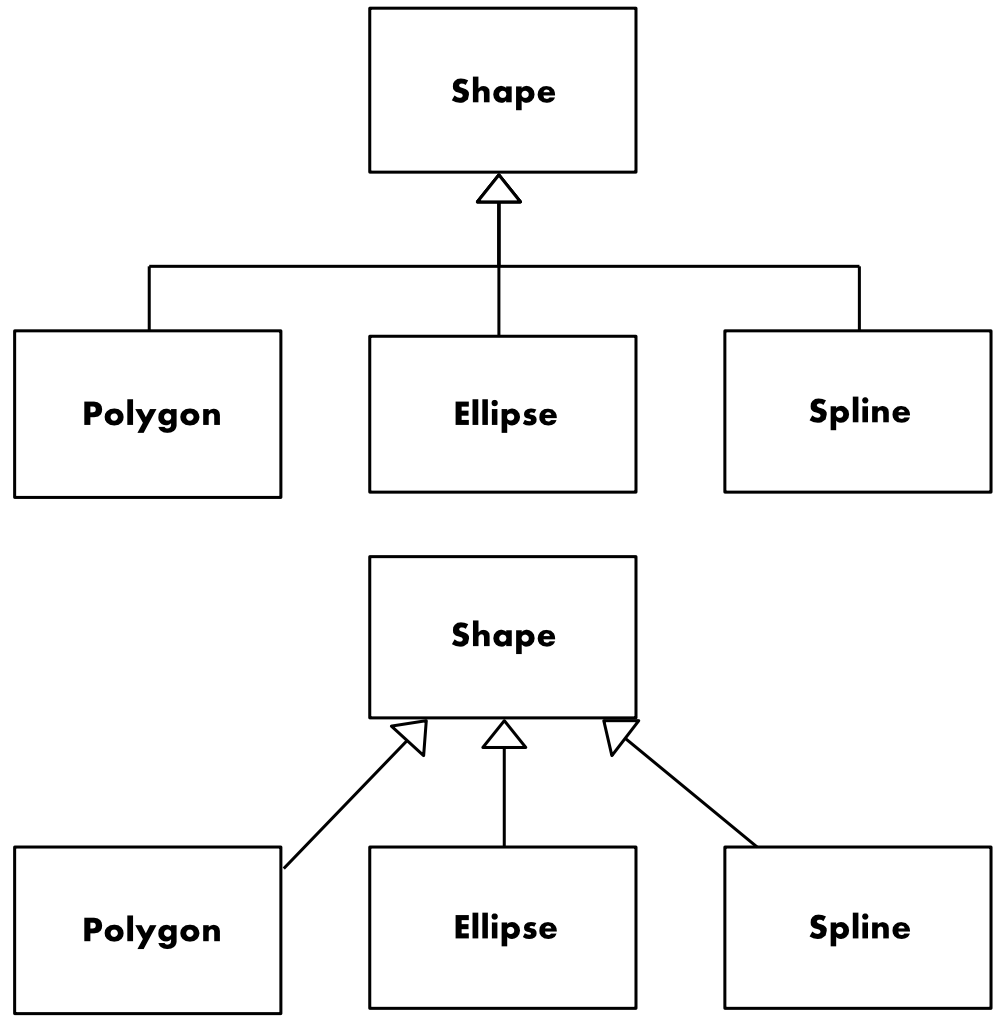
\includegraphics[width=0.5\textwidth]{foto 4.png}
\end{center}
\textit{Nota Bene}: le due soluzioni hanno lo stesso significato, ma il primo è più leggibile.

\subsection*{Dipendenza}
\large

Una dipendenza indica una relazione fornitore/cliente tra elementi del modello in cui \textbf{la modifica di un fornitore può influire sugli elementi del modello del cliente}. Una dipendenza implica che la semantica dei clienti non è completa senza i fornitori.
Una dipendenza viene visualizzata come una freccia tratteggiata tra due classi. La freccia può essere etichettata con una parola chiave o uno stereotipo facoltativo e un nome facoltativo.
\begin{center}
    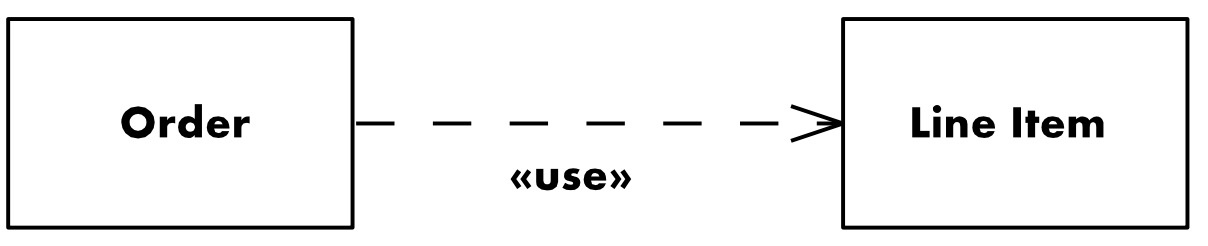
\includegraphics[width=0.5\textwidth]{foto 5.png}
\end{center}
\textit{Nota Bene}: se dovessimo modificare "Line Item" si potrebbe dover modificare anche "Order", data la sua dipendenza da "Line Item".

\subsection*{Realizzazione}
\large

Una realizzazione è una sorta di dipendenza e viene rappresentata graficamente come una linea tratteggiata con una freccia triangolare all'estremità che corrisponde all'elemento realizzato.
Il realizzante deve realizzare, o implementare, il comportamento che l'altro specifica.
\begin{center}
    
\includegraphics[width=0.45\textwidth]{foto 6.png}
\end{center}

\subsection*{Associazione}
\large

Un'associazione afferma che possono esserci collegamenti tra istanze dei tipi associati. Un collegamento è una tupla con un valore per ciascuna estremità dell'associazione. Le associazioni hanno nomi che possono essere visualizzati ed etichette con frecce che aiutano a leggere la direzione dell'etichetta. Le estremità dell'associazione possono avere nomi, molteplicità e frecce o croci di navigazione.
\begin{center}
    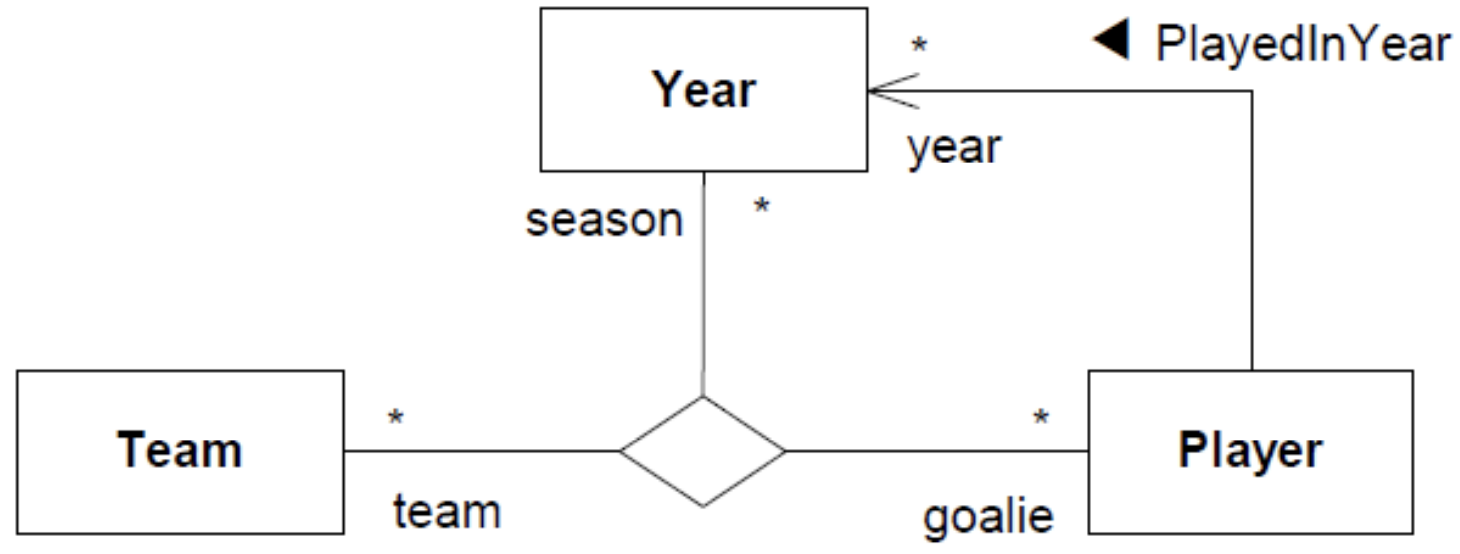
\includegraphics[width=0.7\textwidth]{foto 7.png}
\end{center}
\textit{Spiegazione sintetica}: "PlayedInYear" è una etichetta. Tra Year e Player abbiamo un'associazione binaria, tra Year e Team e Player abbiamo un'associazione ternaria. Osserviamo ora l'associazione tra Player e Year; dato un player si può facilmente risalire agli year corrispondenti, ma non vale il contrario.

\subsection*{Navigazione: frecce e croci}
\large
\begin{center}
    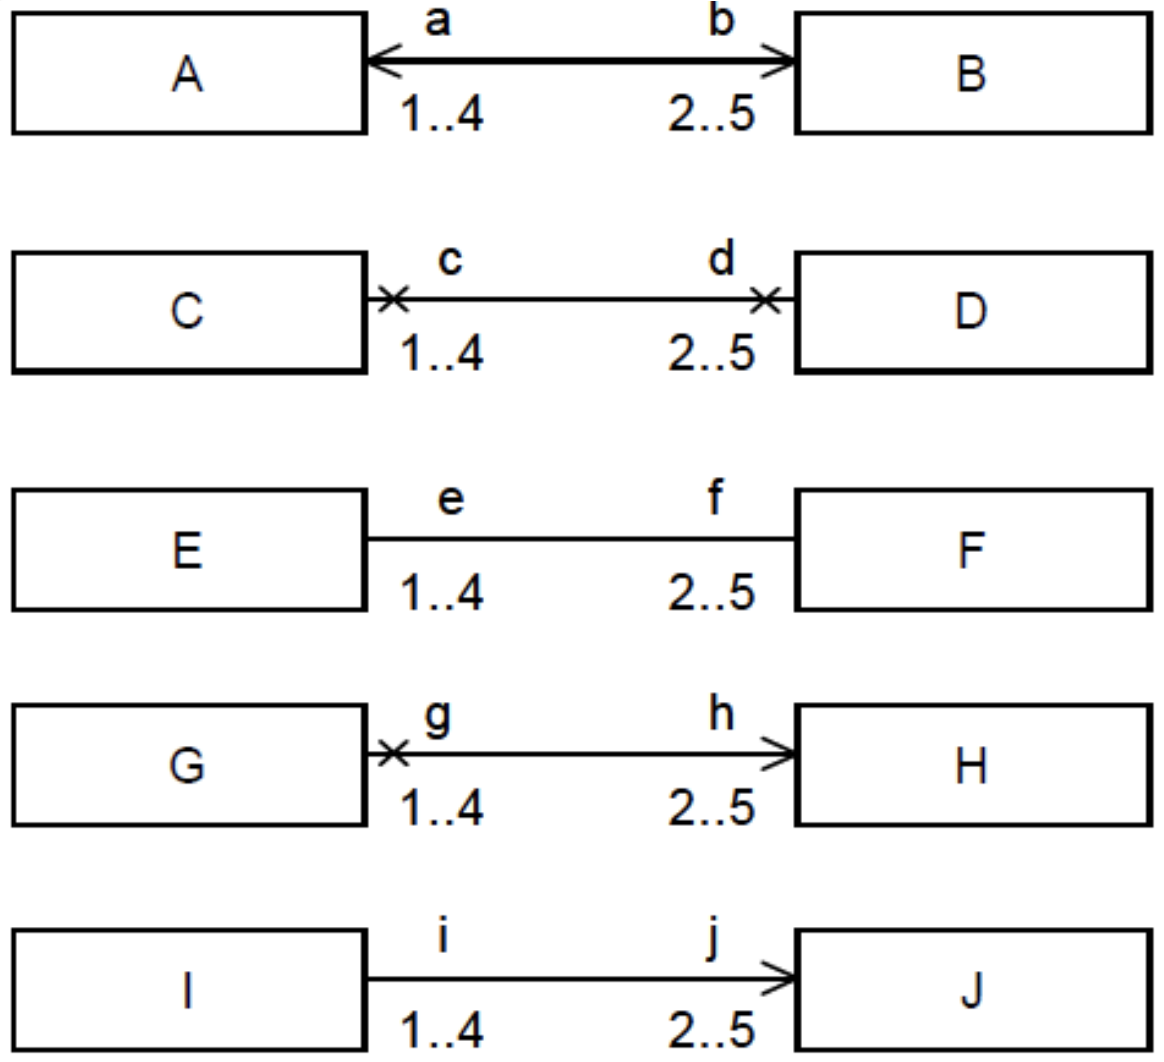
\includegraphics[width=0.55\textwidth]{foto 8.png}
\end{center}
Il numero indica quanti elementi corrispondono agli elementi dell'altro insieme. Le frecce indicano che gli elementi corrispondenti sono facilmente identificabili. In caso di croce invece, non saranno facilmente identificabili. Se non troviamo croci o frecce, non si sa la difficoltà nel trovare gli elementi corrispondenti. Esempio:
\begin{center}
    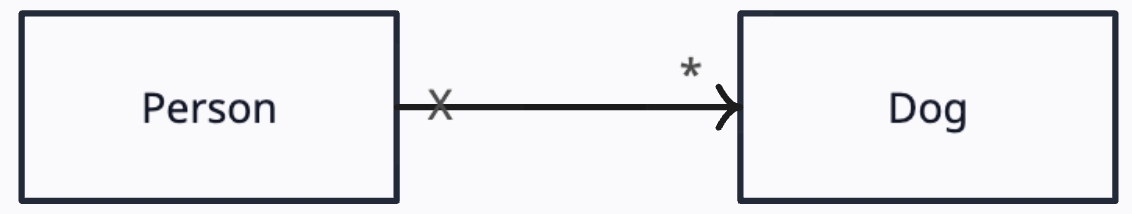
\includegraphics[width=0.55\textwidth]{foto 9.png}
\end{center}
La croce da Person è presente perchè è difficile da un cane risalire al suo padrone, al contrario è più semplice. '*' indica che ogni Person può avere zero o più cani.

\subsection*{Aggregazione}
\large

Un'aggregazione (aggregazione condivisa) ci dice che una parte dell'istanza è indipendente dal composito.
\begin{center}
    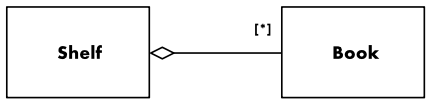
\includegraphics[width=0.55\textwidth]{foto 10.png}
\end{center}

\subsection*{Composizione}
\large

La composizione (aggregazione composita) è un'associazione binaria in parte o per intero. L'oggetto composito è responsabile dell'esistenza e della memorizzazione degli oggetti composti.
\begin{center}
    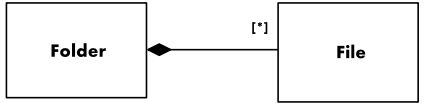
\includegraphics[width=0.55\textwidth]{foto 11.png}
\end{center}

\subsection*{Classi astratte e interfacce}
\large

Una classe astratta non ha istanze dirette: le sue istanze sono istanze di una delle sue specializzazioni. Il nome di una classe astratta è mostrato in \textit{corsivo} o/e utilizzando l'annotazione testuale {abstract}.\vspace{14pt}\\
Le interfacce dichiarano servizi coerenti implementati dalle classi che li implementano. Un'interfaccia specifica un contratto; qualsiasi istanza di una classe che realizza l'interfaccia dovrà adempiere a tale contratto.
\begin{center}
    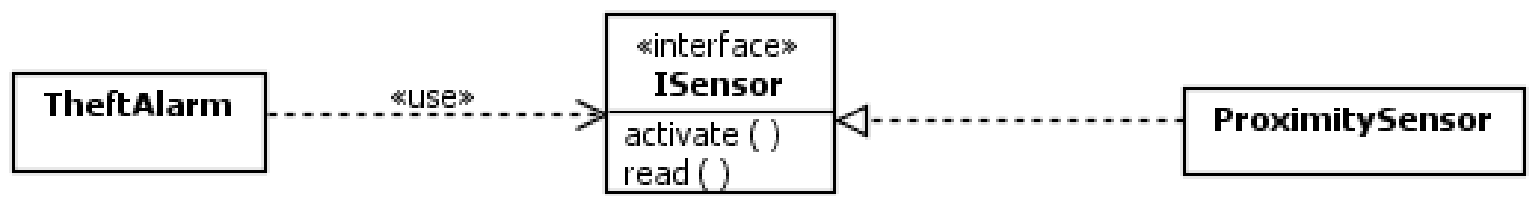
\includegraphics[width=0.75\textwidth]{foto 12.png}
\end{center}

\subsection*{Esempi di modelli di dominio (modello di analisi)}
\large
\begin{center}
    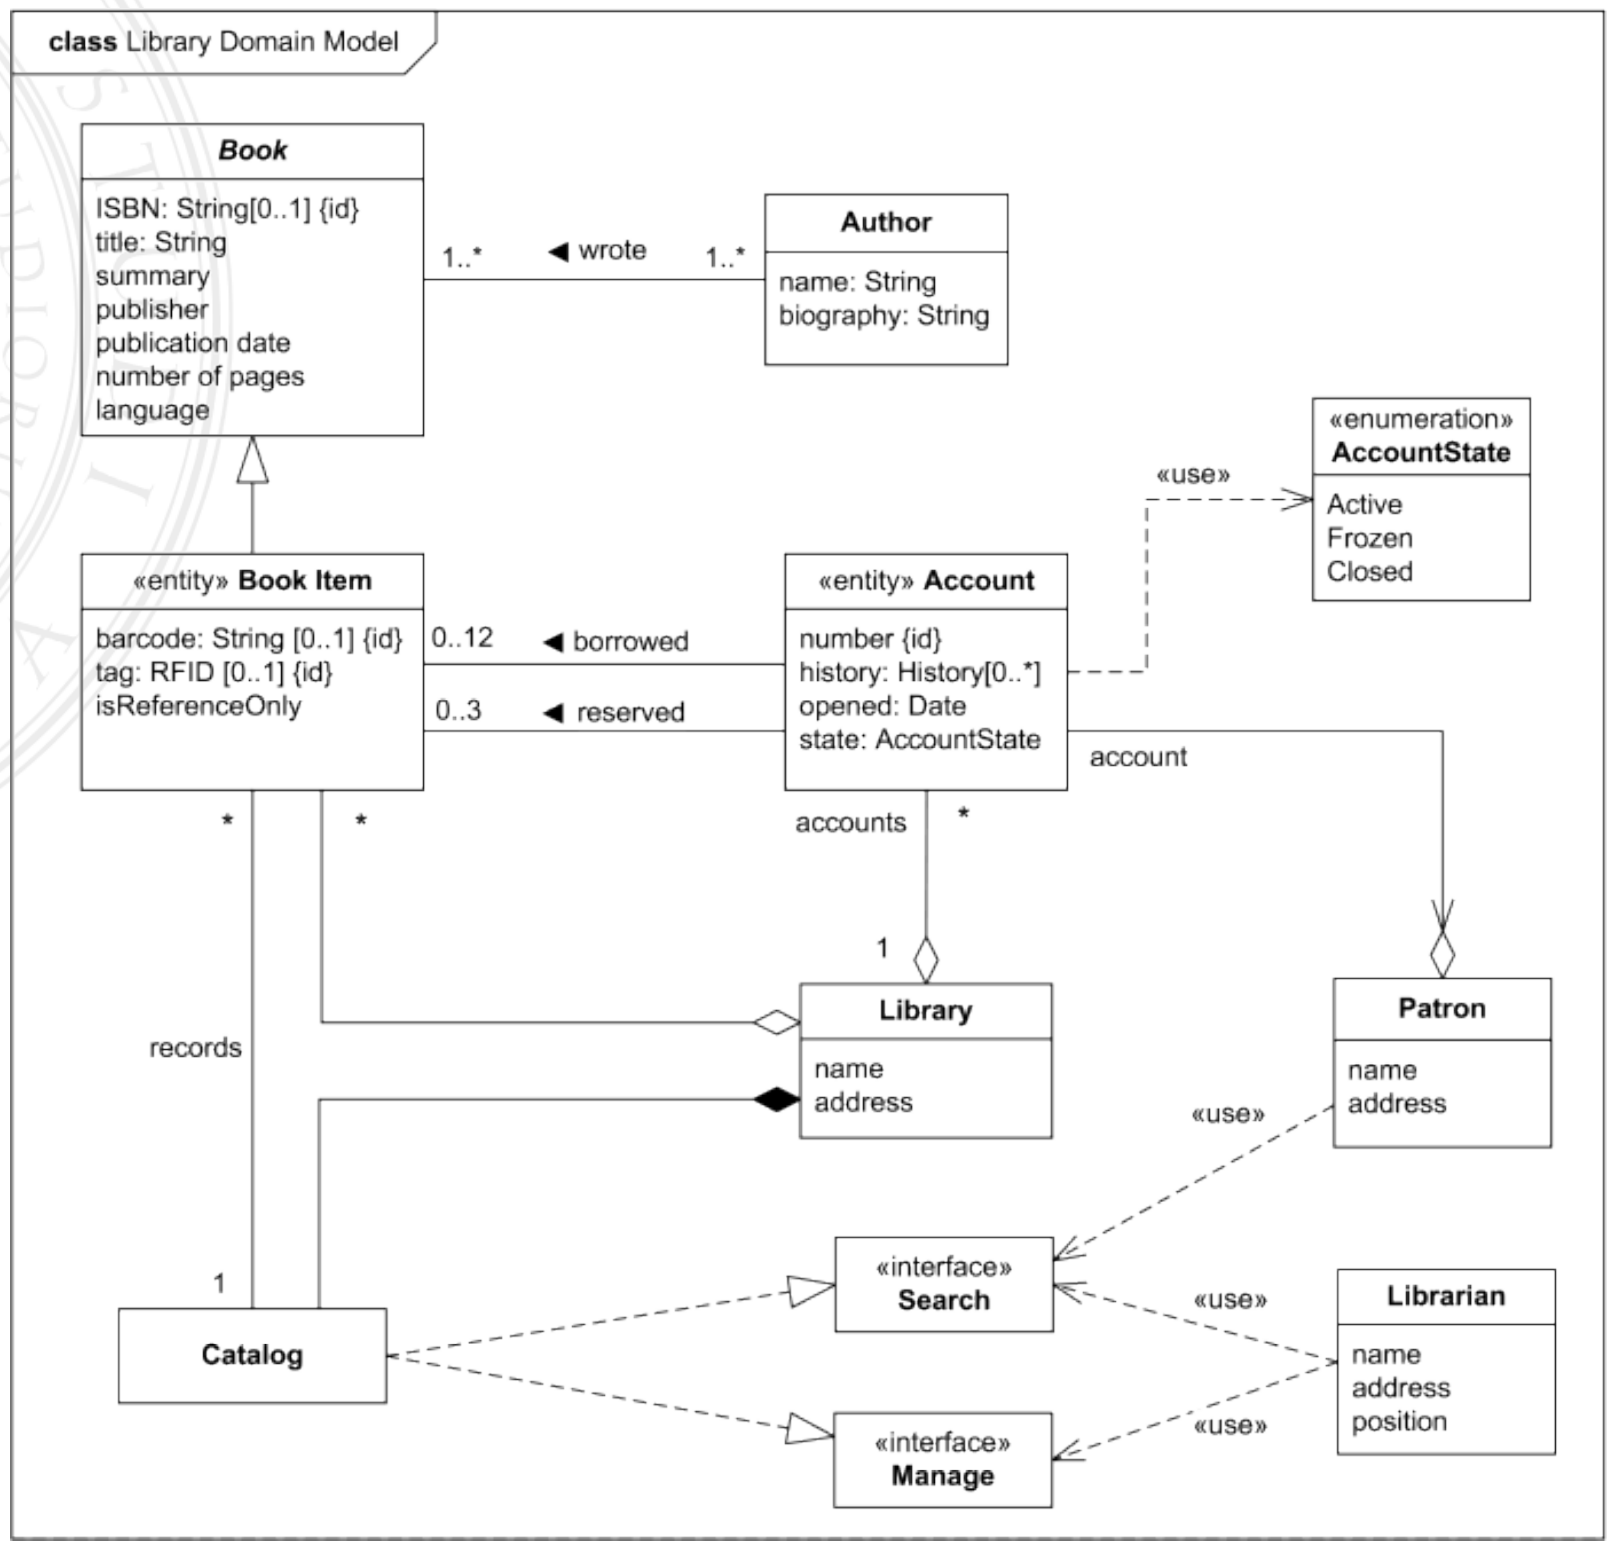
\includegraphics[width=0.75\textwidth]{foto 13.png}
\end{center}
\begin{center}
    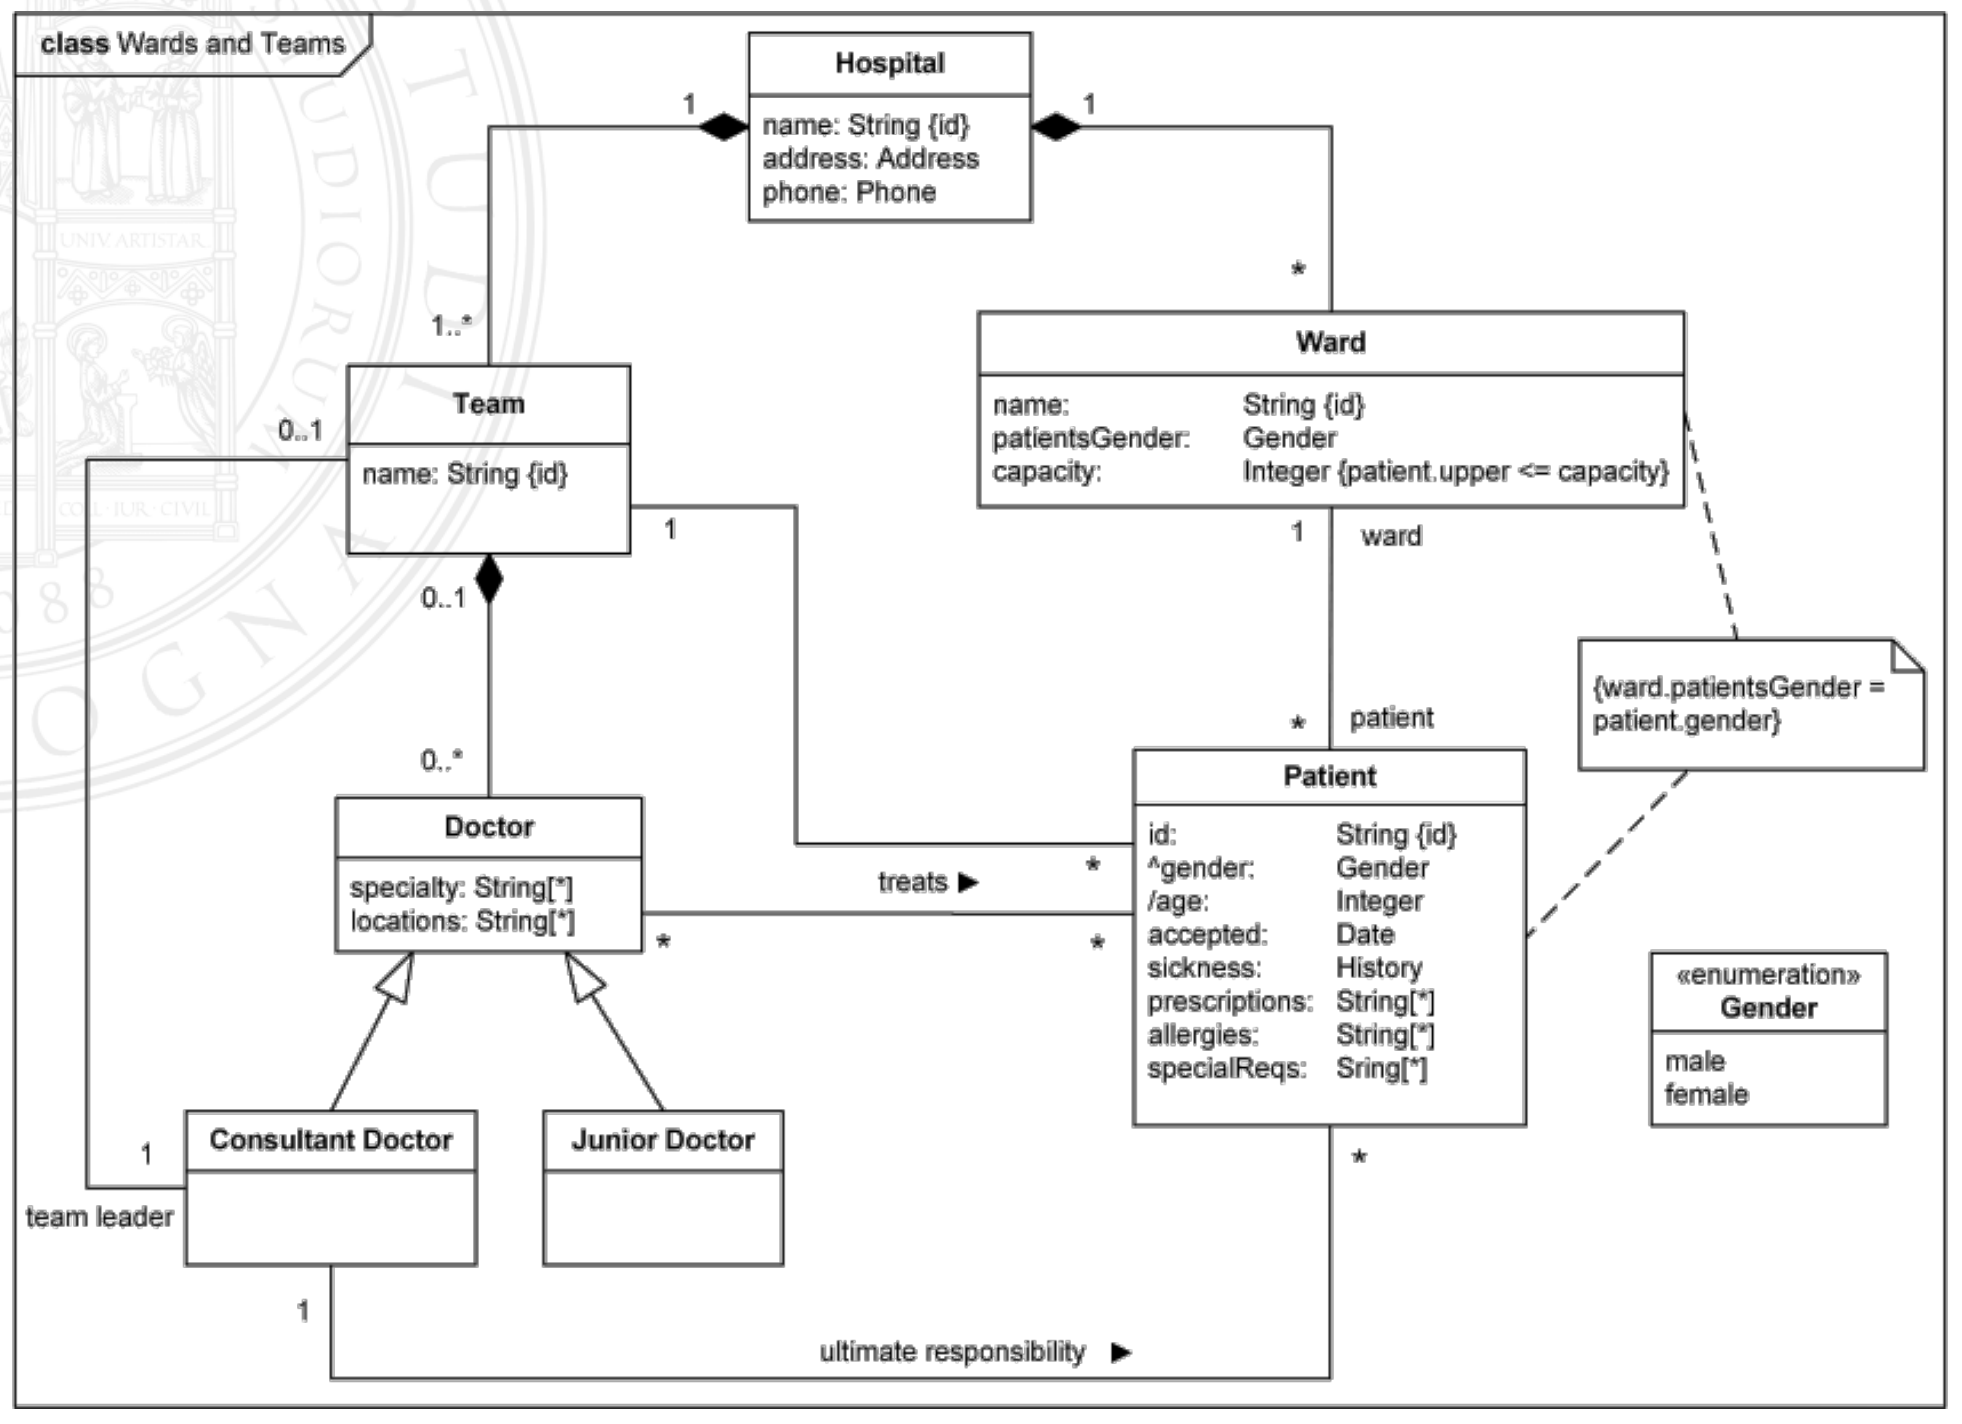
\includegraphics[width=0.75\textwidth]{foto 14.png}
\end{center}

\subsection*{Esempi di modelli di design}
\large
\begin{center}
    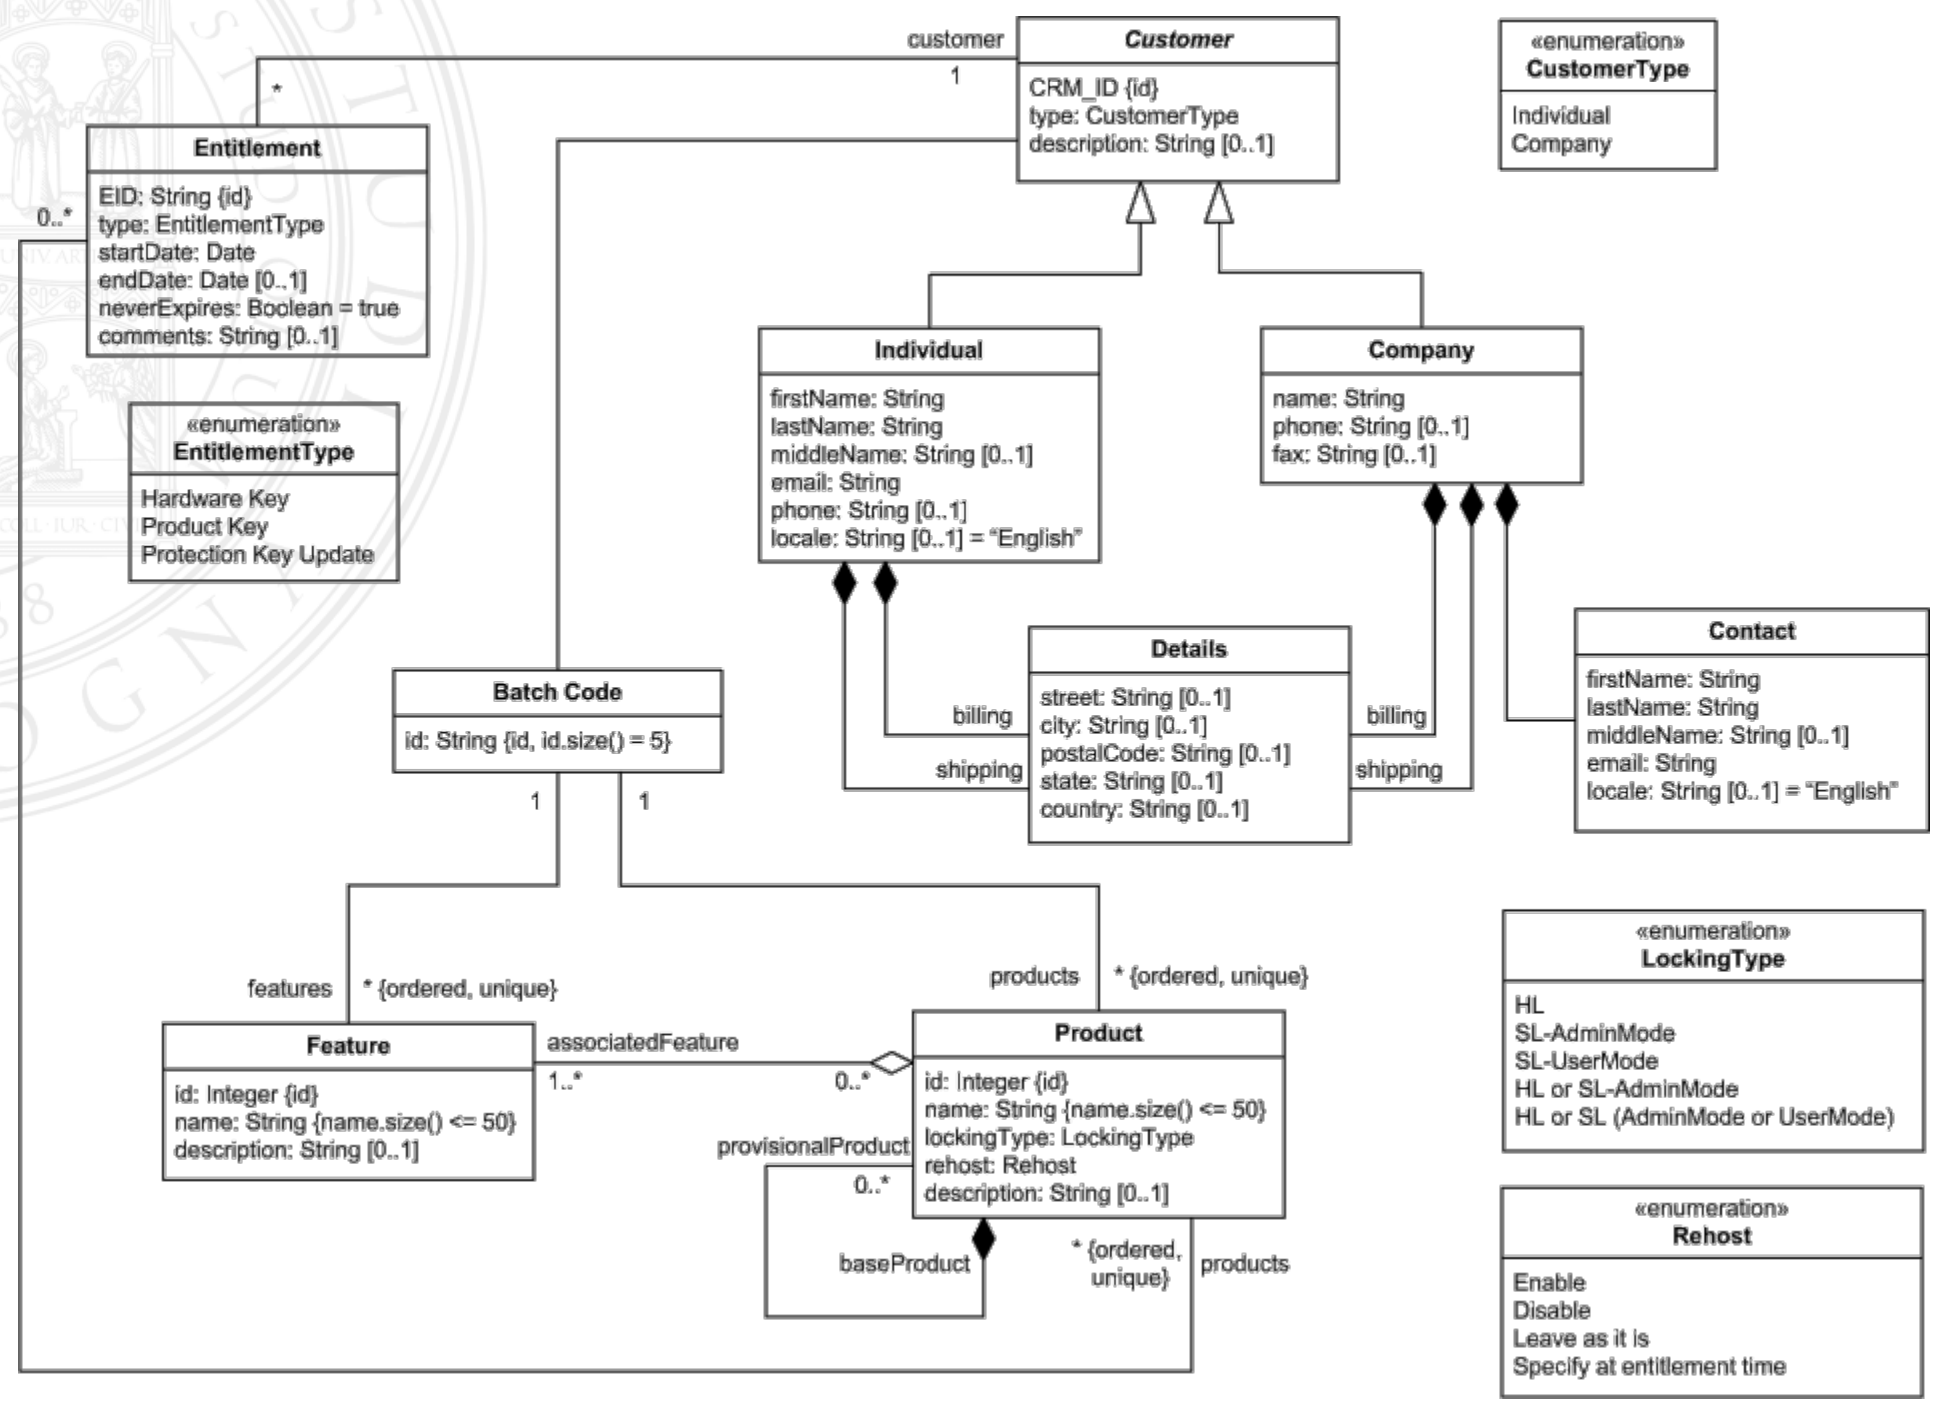
\includegraphics[width=0.75\textwidth]{foto 15.png}
\end{center}

\subsection*{Modello di analisi/dominio}
\large

Nella programmazione Object Oriented il modello di dominio (oggetto) rappresenta il \textbf{concetto} nel dominio del problema, le loro \textbf{caratteristiche} e come si correlano tra loro. È un \textbf{dizionario visivo} per il dominio problematico. \vspace{14pt}\\
L'artefatto risultante è (di solito) un diagramma di classi UML. L'approccio più elementare per identificare le \textbf{classi} inizia con l'analisi di tutti i \textbf{nomi} e le \textbf{frasi nominative} che fanno parte della descrizione del problema. I \textbf{verbi} vengono analizzati successivamente per identificare \textbf{responsabilità e collaborazioni}. Questi passaggi vengono iterati per rifinire il modello (dividere classi, aggregarle, transformarle in proprietà,\dots).

\subsection*{Esercizio}
\large

ciao

\end{document}